\documentclass[10pt]{article}
\usepackage[polish]{babel}
\usepackage[utf8]{inputenc}
\usepackage[T1]{fontenc}
\usepackage{graphicx}
\usepackage[export]{adjustbox}
\graphicspath{ {./images/} }
\usepackage{amsmath}
\usepackage{amsfonts}
\usepackage{amssymb}
\usepackage[version=4]{mhchem}
\usepackage{stmaryrd}
\usepackage{multirow}

\newcommand\Varangle{\mathop{{<\!\!\!\!\!\text{\small)}}\:}\nolimits}

\begin{document}
Arkusz zawiera informacje prawnie chronione do momentu rozpoczęcia egzaminu.

KOD\\
PESEL\\
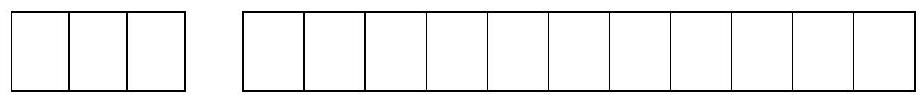
\includegraphics[max width=\textwidth, center]{2024_11_21_779b7f825da3a12753feg-01(1)}\\
\(\square\) dyskalkulia\\

\includegraphics[max width=\textwidth, center]{2024_11_21_779b7f825da3a12753feg-01}\\
\(\square\) dysleksja

\section*{EGZAMIN MATURALNY \\
 Z MATEMATYKI}
\section*{POZIOM PODSTAWOWY}
\section*{Instrukcja dla zdającego}
\begin{enumerate}
  \item Sprawdź, czy arkusz egzaminacyjny zawiera 24 strony (zadania 1-34). Ewentualny brak zgłoś przewodniczącemu zespołu nadzorującego egzamin.
  \item Rozwiązania zadań i odpowiedzi wpisuj w miejscu na to przeznaczonym.
  \item Odpowiedzi do zadań zamkniętych (1-25) zaznacz na karcie odpowiedzi, w części karty przeznaczonej dla zdającego. Zamaluj pola do tego przeznaczone. Błędne zaznaczenie otocz kółkiem \(\bigcirc_{\text {i zaznacz właściwe. }}\)
  \item Pamiętaj, że pominięcie argumentacji lub istotnych obliczeń w rozwiązaniu zadania otwartego (26-34) może spowodować, że za to rozwiązanie nie będziesz mógł dostać pełnej liczby punktów.
  \item Pisz czytelnie i używaj tylko długopisu lub pióra z czarnym tuszem lub atramentem.
  \item Nie używaj korektora, a błędne zapisy wyraźnie przekreśl.
  \item Pamiętaj, że zapisy w brudnopisie nie będą oceniane.
  \item Możesz korzystać z zestawu wzorów matematycznych, cyrkla i linijki oraz kalkulatora prostego.
  \item Na tej stronie oraz na karcie odpowiedzi wpisz swój numer PESEL i przyklej naklejkę z kodem.
  \item Nie wpisuj żadnych znaków w części przeznaczonej dla egzaminatora.
\end{enumerate}

5 MAJA 2016

Godzina rozpoczęcia:\\
9:00

Czas pracy:\\
170 minut

\section*{Liczba punktów do uzyskania: 50}
MMA-P1\_1P-162

\section*{ZADANIA ZAMKNIĘTE}
\section*{W zadaniach od 1. do 25. wybierz izaznacz na karcie odpowiedzi poprawna odpowiedź.}
\section*{Zadanie 1. (1 pkt)}
Dla każdej dodatniej liczby \(a\) iloraz \(\frac{a^{-2,6}}{a^{1,3}}\) jest równy\\
A. \(a^{-3,9}\)\\
B. \(a^{-2}\)\\
C. \(a^{-1,3}\)\\
D. \(a^{1,3}\)

\section*{Zadanie 2. (1 pkt)}
Liczba \(\log _{\sqrt{2}}(2 \sqrt{2})\) jest równa\\
A. \(\frac{3}{2}\)\\
B. 2\\
C. \(\frac{5}{2}\)\\
D. 3

\section*{Zadanie 3. (1 pkt)}
Liczby \(a\) i \(c\) są dodatnie. Liczba \(b\) stanowi 48\% liczby \(a\) oraz 32\% liczby \(c\). Wynika stąd, że\\
A. \(c=1,5 a\)\\
B. \(c=1,6 a\)\\
C. \(c=0,8 a\)\\
D. \(c=0,16 a\)

\section*{Zadanie 4. (1 pkt)}
Równość \((2 \sqrt{2}-a)^{2}=17-12 \sqrt{2}\) jest prawdziwa dla\\
A. \(a=3\)\\
B. \(a=1\)\\
C. \(a=-2\)\\
D. \(a=-3\)

\section*{Zadanie 5. (1 pkt)}
Jedną z liczb, które spełniają nierówność \(-x^{5}+x^{3}-x<-2\), jest\\
A. 1\\
B. -1\\
C. 2\\
D. -2

\section*{Zadanie 6. (1 pkt)}
Proste o równaniach \(2 x-3 y=4\) i \(5 x-6 y=7\) przecinają się w punkcie \(P\). Stąd wynika, że\\
A. \(P=(1,2)\)\\
B. \(P=(-1,2)\)\\
C. \(P=(-1,-2)\)\\
D. \(P=(1,-2)\)

\section*{Zadanie 7. (1 pkt)}
Punkty \(A B C D\) leżą na okręgu o środku \(S\) (zobacz rysunek). Miara kąta \(B D C\) jest równa\\
A. \(91^{\circ}\)\\
B. \(72,5^{\circ}\)\\
C. \(18^{\circ}\)\\
D. \(32^{\circ}\)\\
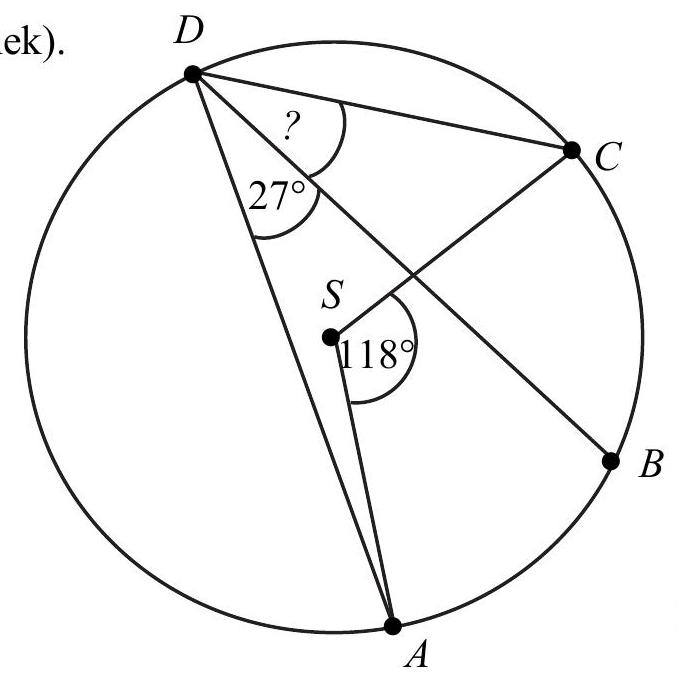
\includegraphics[max width=\textwidth, center]{2024_11_21_779b7f825da3a12753feg-02}

\section*{BRUDNOPIS (nie podlega ocenie)}
\begin{center}

\includegraphics[max width=\textwidth]{2024_11_21_779b7f825da3a12753feg-03}
\end{center}

\section*{Zadanie 8. (1 pkt)}
Dana jest funkcja liniowa \(f(x)=\frac{3}{4} x+6\). Miejscem zerowym tej funkcji jest liczba\\
A. 8\\
B. 6\\
C. -6\\
D. -8

\section*{Zadanie 9. (1 pkt)}
Równanie wymierne \(\frac{3 x-1}{x+5}=3\), gdzie \(x \neq-5\),\\
A. nie ma rozwiązań rzeczywistych.\\
B. ma dokładnie jedno rozwiązanie rzeczywiste.\\
C. ma dokładnie dwa rozwiązania rzeczywiste.\\
D. ma dokładnie trzy rozwiązania rzeczywiste.

\section*{Informacja do zadań 10. i 11.}
Na rysunku przedstawiony jest fragment paraboli będącej wykresem funkcji kwadratowej \(f\). Wierzchołkiem tej paraboli jest punkt \(W=(1,9)\). Liczby -2 i 4 to miejsca zerowe funkcji \(f\).\\
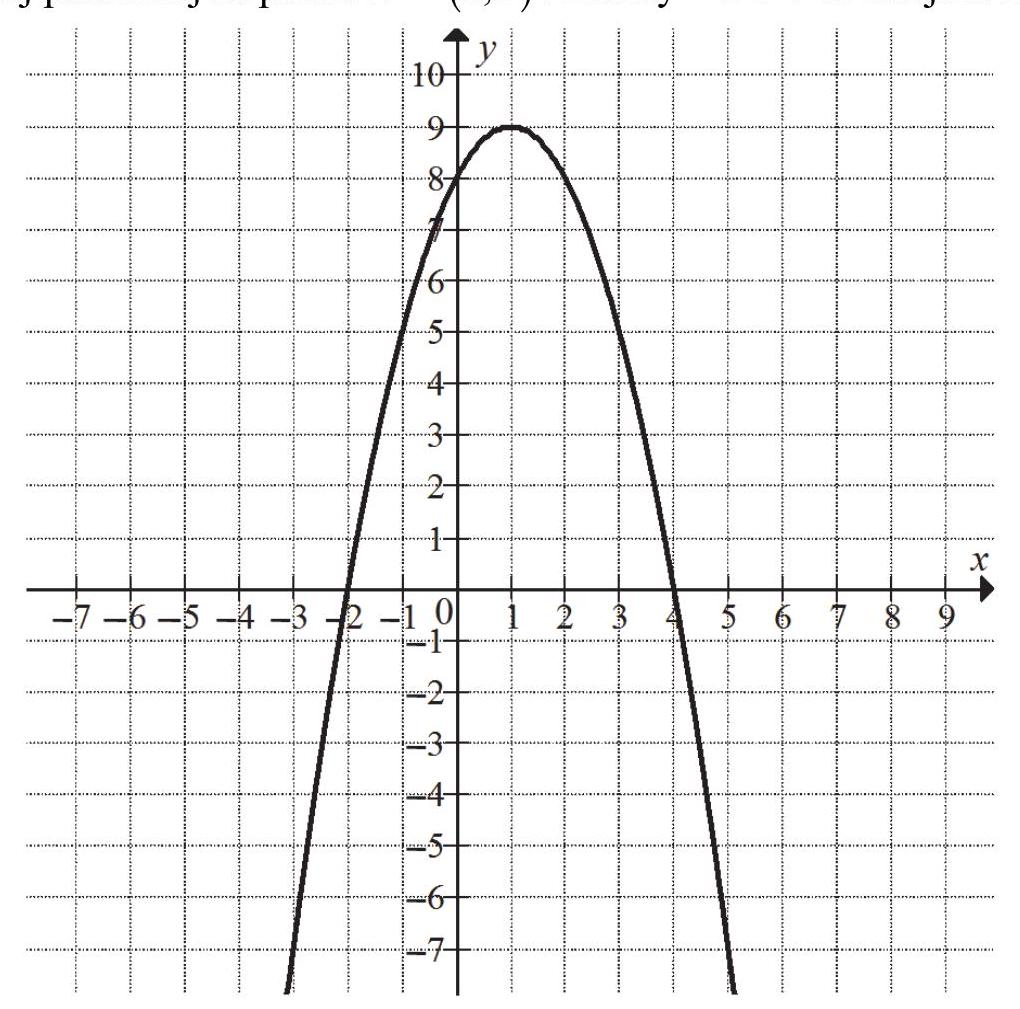
\includegraphics[max width=\textwidth, center]{2024_11_21_779b7f825da3a12753feg-04}

\section*{Zadanie 10. (1 pkt)}
Zbiorem wartości funkcji \(f\) jest przedział\\
A. \((-\infty,-2\rangle\)\\
B. \(\langle-2,4\rangle\)\\
C. \(\langle 4,+\infty)\)\\
D. \((-\infty, 9\rangle\)

\section*{Zadanie 11. (1 pkt)}
Najmniejsza wartość funkcji \(f\) w przedziale \(\langle-1,2\rangle\) jest równa\\
A. 2\\
B. 5\\
C. 8\\
D. 9

\section*{BRUDNOPIS (nie podlega ocenie)}
\begin{center}

\includegraphics[max width=\textwidth]{2024_11_21_779b7f825da3a12753feg-05}
\end{center}

\section*{Zadanie 12. (1 pkt)}
Funkcja \(f\) określona jest wzorem \(f(x)=\frac{2 x^{3}}{x^{6}+1}\) dla każdej liczby rzeczywistej \(x\). Wtedy \(f(-\sqrt[3]{3})\) jest równa\\
A. \(-\frac{\sqrt[3]{9}}{2}\)\\
B. \(-\frac{3}{5}\)\\
C. \(\frac{3}{5}\)\\
D. \(\frac{\sqrt[3]{3}}{2}\)

\section*{Zadanie 13. (1 pkt)}
W okręgu o środku w punkcie \(S\) poprowadzono cięciwę \(A B\), która utworzyła z promieniem \(A S\) kąt o mierze \(31^{\circ}\) (zobacz rysunek). Promień tego okręgu ma długość 10. Odległość punktu \(S\) od cięciwy \(A B\) jest liczbą z przedziału\\
A. \(\left\langle\frac{9}{2}, \frac{11}{2}\right\rangle\)\\
B. \(\left(\frac{11}{2}, \frac{13}{2}\right)\)\\
C. \(\left(\frac{13}{2}, \frac{19}{2}\right)\)\\
D. \(\left(\frac{19}{2}, \frac{37}{2}\right)\)\\
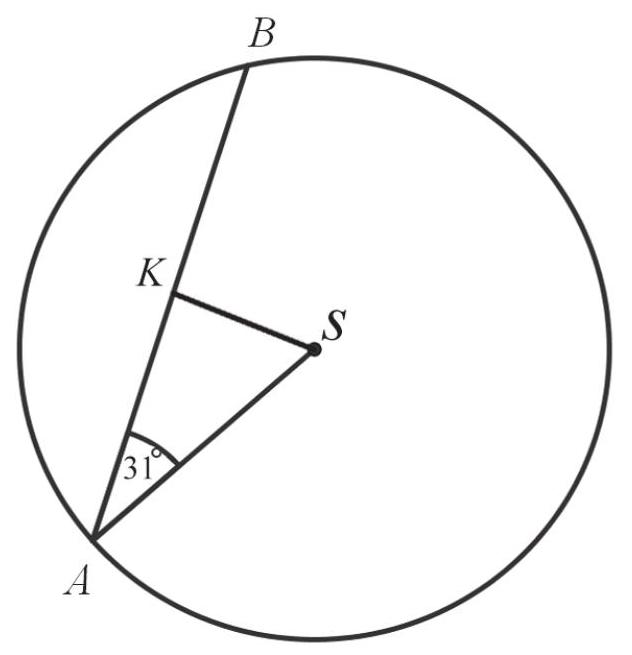
\includegraphics[max width=\textwidth, center]{2024_11_21_779b7f825da3a12753feg-06(1)}

\section*{Zadanie 14. (1 pkt)}
Czternasty wyraz ciągu arytmetycznego jest równy 8 , a różnica tego ciągu jest równa \(\left(-\frac{3}{2}\right)\). Siódmy wyraz tego ciągu jest równy\\
A. \(\frac{37}{2}\)\\
B. \(-\frac{37}{2}\)\\
C. \(-\frac{5}{2}\)\\
D. \(\frac{5}{2}\)

\section*{Zadanie 15. (1 pkt)}
Ciąg \((x, 2 x+3,4 x+3)\) jest geometryczny. Pierwszy wyraz tego ciągu jest równy\\
A. -4\\
B. 1\\
C. 0\\
D. -1

\section*{Zadanie 16. (1 pkt)}
Przedstawione na rysunku trójkąty \(A B C\) i \(P Q R\) są podobne. Bok \(A B\) trójkąta \(A B C\) ma długość\\
A. 8\\
B. 8,5\\
C. 9,5\\
D. 10\\
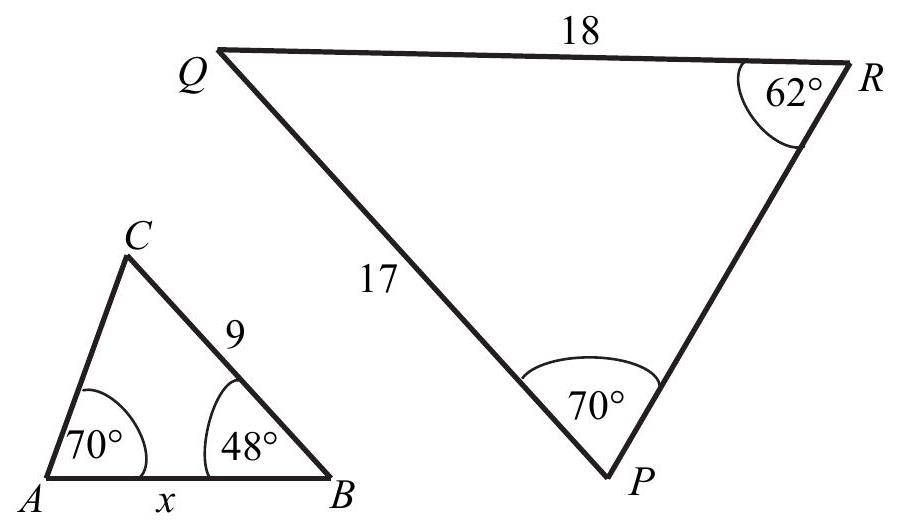
\includegraphics[max width=\textwidth, center]{2024_11_21_779b7f825da3a12753feg-06}

\section*{BRUDNOPIS (nie podlega ocenie)}
\begin{center}

\includegraphics[max width=\textwidth]{2024_11_21_779b7f825da3a12753feg-07}
\end{center}

\section*{Zadanie 17. (1 pkt)}
Kąt \(\alpha\) jest ostry i \(\operatorname{tg} \alpha=\frac{2}{3}\). Wtedy\\
A. \(\sin \alpha=\frac{3 \sqrt{13}}{26}\)\\
B. \(\sin \alpha=\frac{\sqrt{13}}{13}\)\\
C. \(\sin \alpha=\frac{2 \sqrt{13}}{13}\)\\
D. \(\sin \alpha=\frac{3 \sqrt{13}}{13}\)

\section*{Zadanie 18. (1 pkt)}
Z odcinków o długościach: \(5,2 a+1, a-1\) można zbudować trójkąt równoramienny. Wynika stąd, że\\
A. \(a=6\)\\
B. \(a=4\)\\
C. \(a=3\)\\
D. \(a=2\)

\section*{Zadanie 19. (1 pkt)}
Okręgi o promieniach 3 i 4 są styczne zewnętrznie. Prosta styczna do okręgu o promieniu 4 w punkcie \(P\) przechodzi przez środek okręgu o promieniu 3 (zobacz rysunek).\\
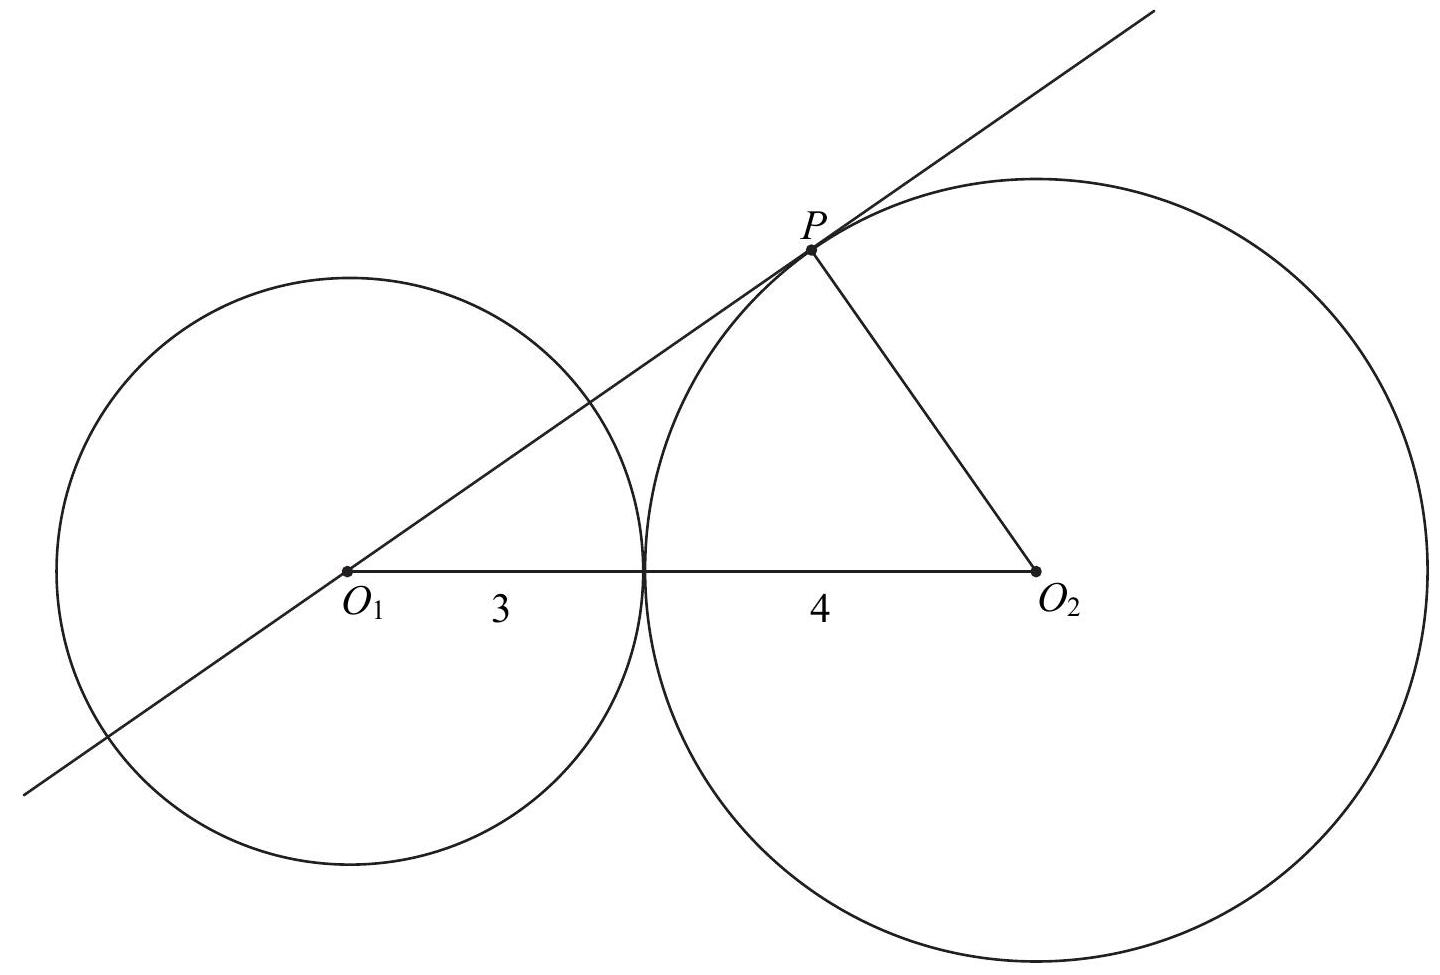
\includegraphics[max width=\textwidth, center]{2024_11_21_779b7f825da3a12753feg-08}

Pole trójkąta, którego wierzchołkami są środki okręgów i punkt styczności \(P\), jest równe\\
A. 14\\
B. \(2 \sqrt{33}\)\\
C. \(4 \sqrt{33}\)\\
D. 12

\section*{Zadanie 20. (1 pkt)}
Proste opisane równaniami \(y=\frac{2}{m-1} x+m-2\) oraz \(y=m x+\frac{1}{m+1}\) są prostopadłe, gdy\\
A. \(m=2\)\\
B. \(m=\frac{1}{2}\)\\
C. \(m=\frac{1}{3}\)\\
D. \(m=-2\)

\section*{BRUDNOPIS (nie podlega ocenie)}
\(\qquad\)

\section*{Zadanie 21. (1 pkt)}
W układzie współrzędnych dane są punkty \(A=(a, 6)\) oraz \(B=(7, b)\). Środkiem odcinka \(A B\) jest punkt \(M=(3,4)\). Wynika stąd, że\\
A. \(a=5\) i \(b=5\)\\
B. \(\quad a=-1\) i \(b=2\)\\
C. \(a=4\) i \(b=10\)\\
D. \(a=-4\) i \(b=-2\)

\section*{Zadanie 22. (1 pkt)}
Rzucamy trzy razy symetryczną monetą. Niech \(p\) oznacza prawdopodobieństwo otrzymania dokładnie dwóch orłów w tych trzech rzutach. Wtedy\\
A. \(0 \leq p<0,2\)\\
B. \(0,2 \leq p \leq 0,35\)\\
C. \(0,35<p \leq 0,5\)\\
D. \(0,5<p \leq 1\)

\section*{Zadanie 23. (1 pkt)}
Kąt rozwarcia stożka ma miarę \(120^{\circ}\), a tworząca tego stożka ma długość 4 . Objętość tego stożka jest równa\\
A. \(36 \pi\)\\
B. \(18 \pi\)\\
C. \(24 \pi\)\\
D. \(8 \pi\)

\section*{Zadanie 24. (1 pkt)}
Przekątna podstawy graniastosłupa prawidłowego czworokątnego jest dwa razy dłuższa od wysokości graniastosłupa. Graniastosłup przecięto płaszczyzną przechodzącą przez przekątną podstawy i jeden wierzchołek drugiej podstawy (patrz rysunek).\\
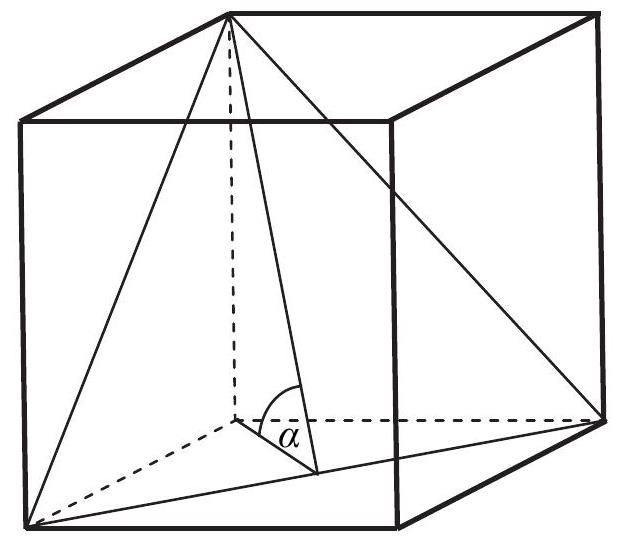
\includegraphics[max width=\textwidth, center]{2024_11_21_779b7f825da3a12753feg-10}

Płaszczyzna przekroju tworzy z podstawą graniastosłupa kąt \(\alpha\) o mierze\\
A. \(30^{\circ}\)\\
B. \(45^{\circ}\)\\
C. \(60^{\circ}\)\\
D. \(75^{\circ}\)

\section*{Zadanie 25. (1 pkt)}
Średnia arytmetyczna sześciu liczb naturalnych: \(31,16,25,29,27, x\), jest równa \(\frac{x}{2}\). Mediana tych liczb jest równa\\
A. 26\\
B. 27\\
C. 28\\
D. 29

\section*{BRUDNOPIS (nie podlega ocenie)}
\begin{center}

\includegraphics[max width=\textwidth]{2024_11_21_779b7f825da3a12753feg-11}
\end{center}

\section*{ZADANIA OTWARTE}
Rozwiąania zadań o numerach od 26. do 34. należ̀y zapisać w wyznaczonych miejscach pod treścią zadania.

\section*{Zadanie 26. (2 pkt)}
Rozwiąż nierówność \(2 x^{2}+5 x-3>0\).\\

\includegraphics[max width=\textwidth, center]{2024_11_21_779b7f825da3a12753feg-12}

\section*{Zadanie 27. (2 pkt)}
Rozwiąż równanie \(x^{3}+3 x^{2}+2 x+6=0\).\\

\includegraphics[max width=\textwidth, center]{2024_11_21_779b7f825da3a12753feg-13}

Odpowiedź:

\begin{center}
\begin{tabular}{|c|l|c|c|}
\hline
\multirow{2}{*}{\begin{tabular}{c}
Wypelnia \\
egzaminator \\
\end{tabular}} & Nr zadania & 26. & 27. \\
\cline { 2 - 4 }
 & Maks. liczba pkt & \(\mathbf{2}\) & \(\mathbf{2}\) \\
\cline { 2 - 4 }
 & Uzyskana liczba pkt &  &  \\
\hline
\end{tabular}
\end{center}

\section*{Zadanie 28. (2 pkt)}
Kąt \(\alpha\) jest ostry i \((\sin \alpha+\cos \alpha)^{2}=\frac{3}{2}\). Oblicz wartość wyrażenia \(\sin \alpha \cdot \cos \alpha\).\\

\includegraphics[max width=\textwidth, center]{2024_11_21_779b7f825da3a12753feg-14}

Odpowiedź:

\section*{Zadanie 29. (2 pkt)}
Dany jest trójkąt prostokątny \(A B C\). Na przyprostokątnych \(A C\) i \(A B\) tego trójkąta obrano odpowiednio punkty \(D\) i \(G\). Na przeciwprostokątnej \(B C\) wyznaczono punkty \(E\) i \(F\) takie, że \(|\Varangle D E C|=|\Varangle B G F|=90^{\circ}\) (zobacz rysunek). Wykaż, że trójkąt CDE jest podobny do trójkąta \(F B G\).\\
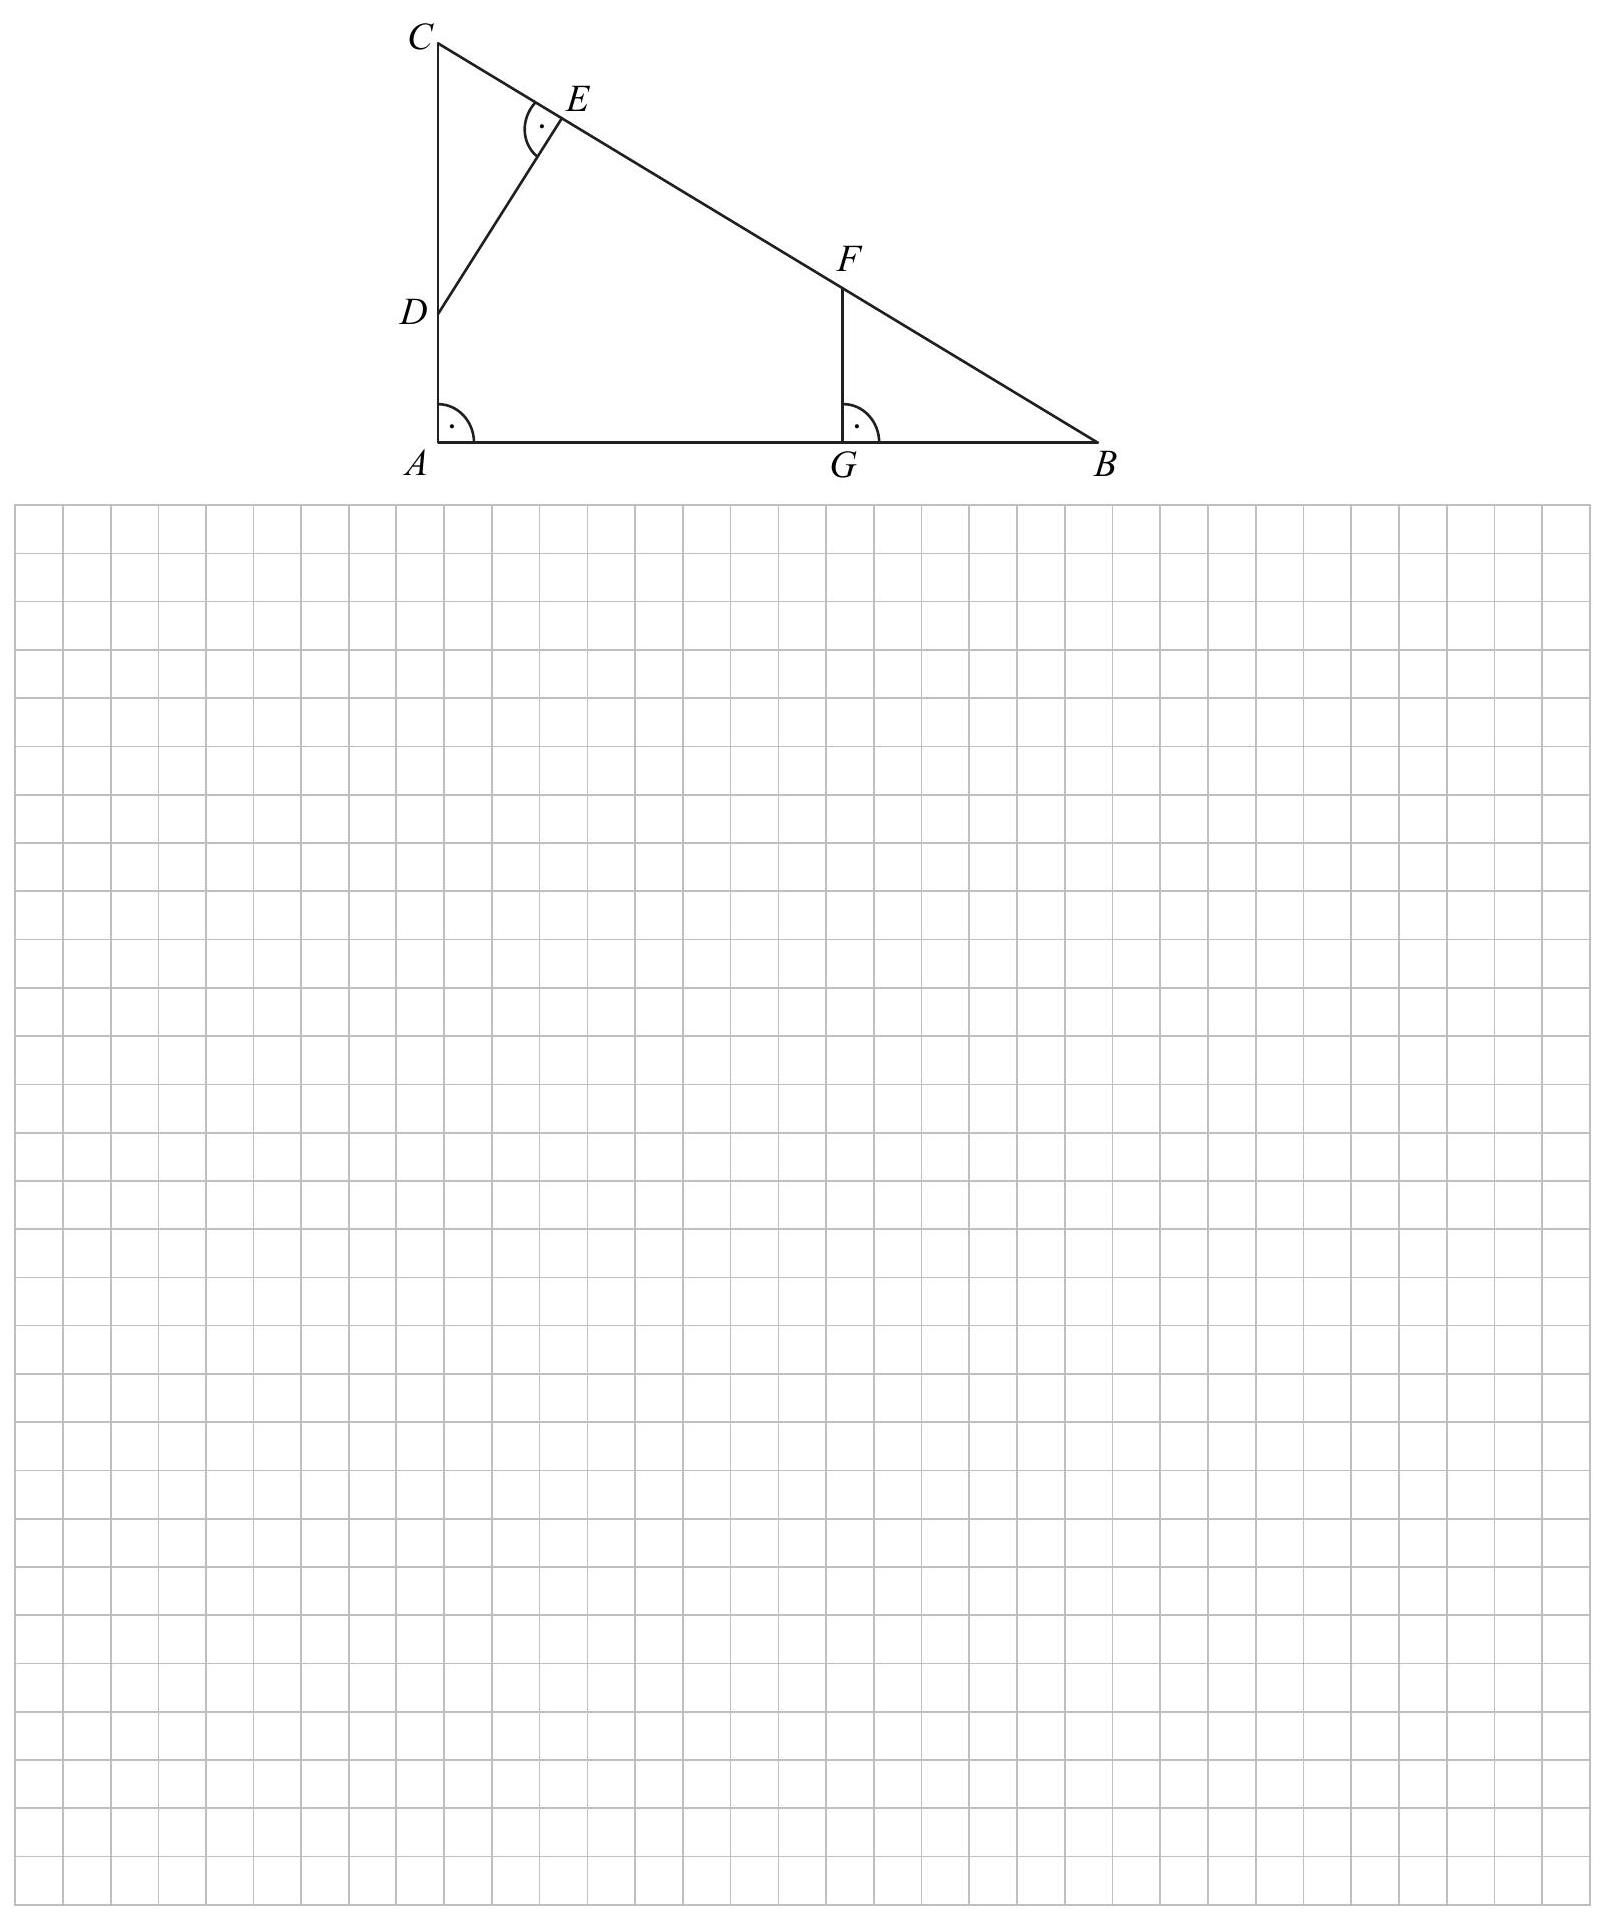
\includegraphics[max width=\textwidth, center]{2024_11_21_779b7f825da3a12753feg-15}

\begin{center}
\begin{tabular}{|c|l|c|c|}
\hline
\multirow{2}{*}{\begin{tabular}{l}
Wypełnia \\
egzaminator \\
\end{tabular}} & Nr zadania & 28. & 29. \\
\cline { 2 - 4 }
 & Maks. liczba pkt & 2 & 2 \\
\cline { 2 - 4 }
 & Uzyskana liczba pkt &  &  \\
\hline
\end{tabular}
\end{center}

\section*{Zadanie 30. (2 pkt)}
Ciąg \(\left(a_{n}\right)\) jest określony wzorem \(a_{n}=2 n^{2}+2 n\) dla \(n \geq 1\). Wykaż, że suma każdych dwóch kolejnych wyrazów tego ciągu jest kwadratem liczby naturalnej.\\

\includegraphics[max width=\textwidth, center]{2024_11_21_779b7f825da3a12753feg-16}

\section*{Zadanie 31. (2 pkt)}
W skończonym ciągu arytmetycznym \(\left(a_{n}\right)\) pierwszy wyraz \(a_{1}\) jest równy 7 oraz ostatni wyraz \(a_{n}\) jest równy 89. Suma wszystkich wyrazów tego ciągu jest równa 2016.\\
Oblicz, ile wyrazów ma ten ciąg.\\

\includegraphics[max width=\textwidth, center]{2024_11_21_779b7f825da3a12753feg-17}

Odpowiedź:

\begin{center}
\begin{tabular}{|c|l|c|c|}
\hline
\multirow{3}{*}{\begin{tabular}{l}
Wypelnia \\
egzaminator \\
\end{tabular}} & Nr zadania & 30. & 31. \\
\cline { 2 - 4 }
 & Maks. liczba pkt & \(\mathbf{2}\) & \(\mathbf{2}\) \\
\cline { 2 - 4 }
 & Uzyskana liczba pkt &  &  \\
\hline
\end{tabular}
\end{center}

\section*{Zadanie 32. (4 pkt)}
Jeden z kątów trójkąta jest trzy razy większy od mniejszego z dwóch pozostałych kątów, które różnią się o \(50^{\circ}\). Oblicz kąty tego trójkąta.\\

\includegraphics[max width=\textwidth, center]{2024_11_21_779b7f825da3a12753feg-18}\\

\includegraphics[max width=\textwidth, center]{2024_11_21_779b7f825da3a12753feg-19}

Odpowiedź:

\begin{center}
\begin{tabular}{|c|l|c|}
\hline
\multirow{2}{*}{\begin{tabular}{c}
Wypetnia \\
egzaminator \\
\end{tabular}} & Nr zadania & 32. \\
\cline { 2 - 3 }
 & Maks. liczba pkt & 4 \\
\cline { 2 - 3 }
 & Uzyskana liczba pkt &  \\
\hline
\end{tabular}
\end{center}

\section*{Zadanie 33. (5 pkt)}
Grupa znajomych wyjeżdżających na biwak wynajęła bus. Koszt wynajęcia busa jest równy 960 złotych i tę kwotę rozłożono po równo pomiędzy uczestników wyjazdu. Do grupy wyjeżdżających dołączyło w ostatniej chwili dwóch znajomych. Wtedy koszt wyjazdu przypadający na jednego uczestnika zmniejszył się o 16 złotych. Oblicz, ile osób wyjechało na biwak.\\

\includegraphics[max width=\textwidth, center]{2024_11_21_779b7f825da3a12753feg-20}\\

\includegraphics[max width=\textwidth, center]{2024_11_21_779b7f825da3a12753feg-21}

\begin{center}
\begin{tabular}{|c|l|c|}
\hline
\multirow{2}{*}{\begin{tabular}{c}
Wypetnia \\
egzaminator \\
\end{tabular}} & Nr zadania & 33. \\
\cline { 2 - 3 }
 & Maks. liczba pkt & 5 \\
\cline { 2 - 3 }
 & Uzyskana liczba pkt &  \\
\hline
\end{tabular}
\end{center}

\section*{Zadanie 34. (4 pkt)}
Ze zbioru wszystkich liczb naturalnych dwucyfrowych losujemy kolejno dwa razy po jednej liczbie bez zwracania. Oblicz prawdopodobieństwo zdarzenia polegającego na tym, że suma wylosowanych liczb będzie równa 30. Wynik zapisz w postaci ułamka zwykłego nieskracalnego.\\

\includegraphics[max width=\textwidth, center]{2024_11_21_779b7f825da3a12753feg-22}\\

\includegraphics[max width=\textwidth, center]{2024_11_21_779b7f825da3a12753feg-23}

Odpowiedź: \(\qquad\)

\begin{center}
\begin{tabular}{|c|l|c|}
\hline
\multirow{2}{*}{\begin{tabular}{c}
Wypetnia \\
egzaminator \\
\end{tabular}} & Nr zadania & 34. \\
\cline { 2 - 3 }
 & Maks. liczba pkt & 4 \\
\cline { 2 - 3 }
 & Uzyskana liczba pkt &  \\
\hline
\end{tabular}
\end{center}

\section*{BRUDNOPIS (nie podlega ocenie)}

\end{document}